\documentclass[a4paper,10pt,english]{article}
%\documentclass[12pt,preprint]{aastex}
\usepackage[utf8]{inputenc}
\usepackage[margin=0.5in]{geometry} % narrow margins
\usepackage{multicol}
% Document formatting
\setlength{\parindent}{0mm}
\setlength{\parskip}{1.5mm}

\usepackage{amsfonts}
\usepackage{graphicx}
\usepackage{float}
\usepackage{cite}
\usepackage{amsmath}
\usepackage{epsfig,floatflt}
\usepackage{hyperref}
\usepackage{listings}
\usepackage[table,xcdraw]{xcolor}
\usepackage{booktabs}
\usepackage{subfig}
\usepackage{algpseudocode}
\usepackage{algorithm}
%\usepackage{amsmath,graphicx,varioref,verbatim,amsfonts,geometry,amssymb,dsfont,blindtext}
\hypersetup{colorlinks=true}
\usepackage{xcolor}
\usepackage{hhline}
\usepackage[export]{adjustbox}
\definecolor{LightGray}{gray}{0.95}
\definecolor{dkgreen}{rgb}{0,0.6,0}
\definecolor{gray}{rgb}{0.5,0.5,0.5}
\definecolor{mauve}{rgb}{0.58,0,0.82}
\definecolor{mygray}{rgb}{0.9,0.9,0.9}
\definecolor{LightGray}{gray}{0.95}
\lstset{frame=tb,
	language=Python,
	aboveskip=3mm,
	belowskip=3mm,
	showstringspaces=false,
	columns=flexible,
	basicstyle={\small\ttfamily},
	numbers=none,
	numberstyle=\tiny\color{gray},
	keywordstyle=\color{blue},
	commentstyle=\color{dkgreen},
	stringstyle=\color{mauve},
	backgroundcolor=\color{mygray},
	breaklines=true,
	postbreak=\mbox{\textcolor{red}{$\hookrightarrow$}\space}
	%breakatwhitespace=true,
	%tabsize=3
}

%\usepackage[english]{babel}
%\usepackage{fancyhdr}
%\usepackage{lastpage}
%
%\pagestyle{fancy}
%\fancyhf{}
%
%\rfoot{Page \thepage \hspace{1pt} of \pageref{LastPage}}
\pagenumbering{arabic}

\begin{document}
\title{FYS-STK4155 Project 2}
\author{Bendik Steinsvåg Dalen \& Gabriel Sigurd Cabrera}
%\maketitle

\maketitle
\begin{abstract}
\end{abstract}

\begin{multicols*}{2}

\section*{Introduction}
\label{sec:introduction}

\section*{Data}
\label{sec:data}

\subsection*{Credit Card Data}

Our first dataset contains real credit card metadata for 30,000 people, in the form of a \texttt{.xls} file; each given datapoint (or person) has 23 features and one \textit{binary output} denoting whether or not they've defaulted on their credit card debt.  These features can be summarized as follows:

\begin{enumerate}
\item 
\end{enumerate}

\subsection*{The Franke Function}

The second dataset will be given by the \textit{Franke function}, which is defined as follows:

\begin{align*}
f(x,y) &= \frac{3}{4} \exp \left( -\frac{(9x-2)^2}{4} -\frac{(9y-2)^2}{4} \right) \\ &+ \frac{3}{4} \exp \left( -\frac{9x+1}{49} -\frac{9y+1}{10} \right) \\ &+ \frac{1}{2} \exp \left( -\frac{(9x-7)^2}{4} -\frac{(9y-3)^2}{4} \right) \\ &- \frac{1}{5} \exp \left( -(9x-4)^2 - (9y-7)^2 \right)
\end{align*}

We will be solving the Franke function for 100 $x$-values and 100 $y$-values in the range $[0,1]$, leaving us with a grid containing a total of 10000 $xy$ coordinate pairs.  This leaves us with the values plotted in Figure \ref{fig_Franke}.

\begin{figure}[H]
	\centering
	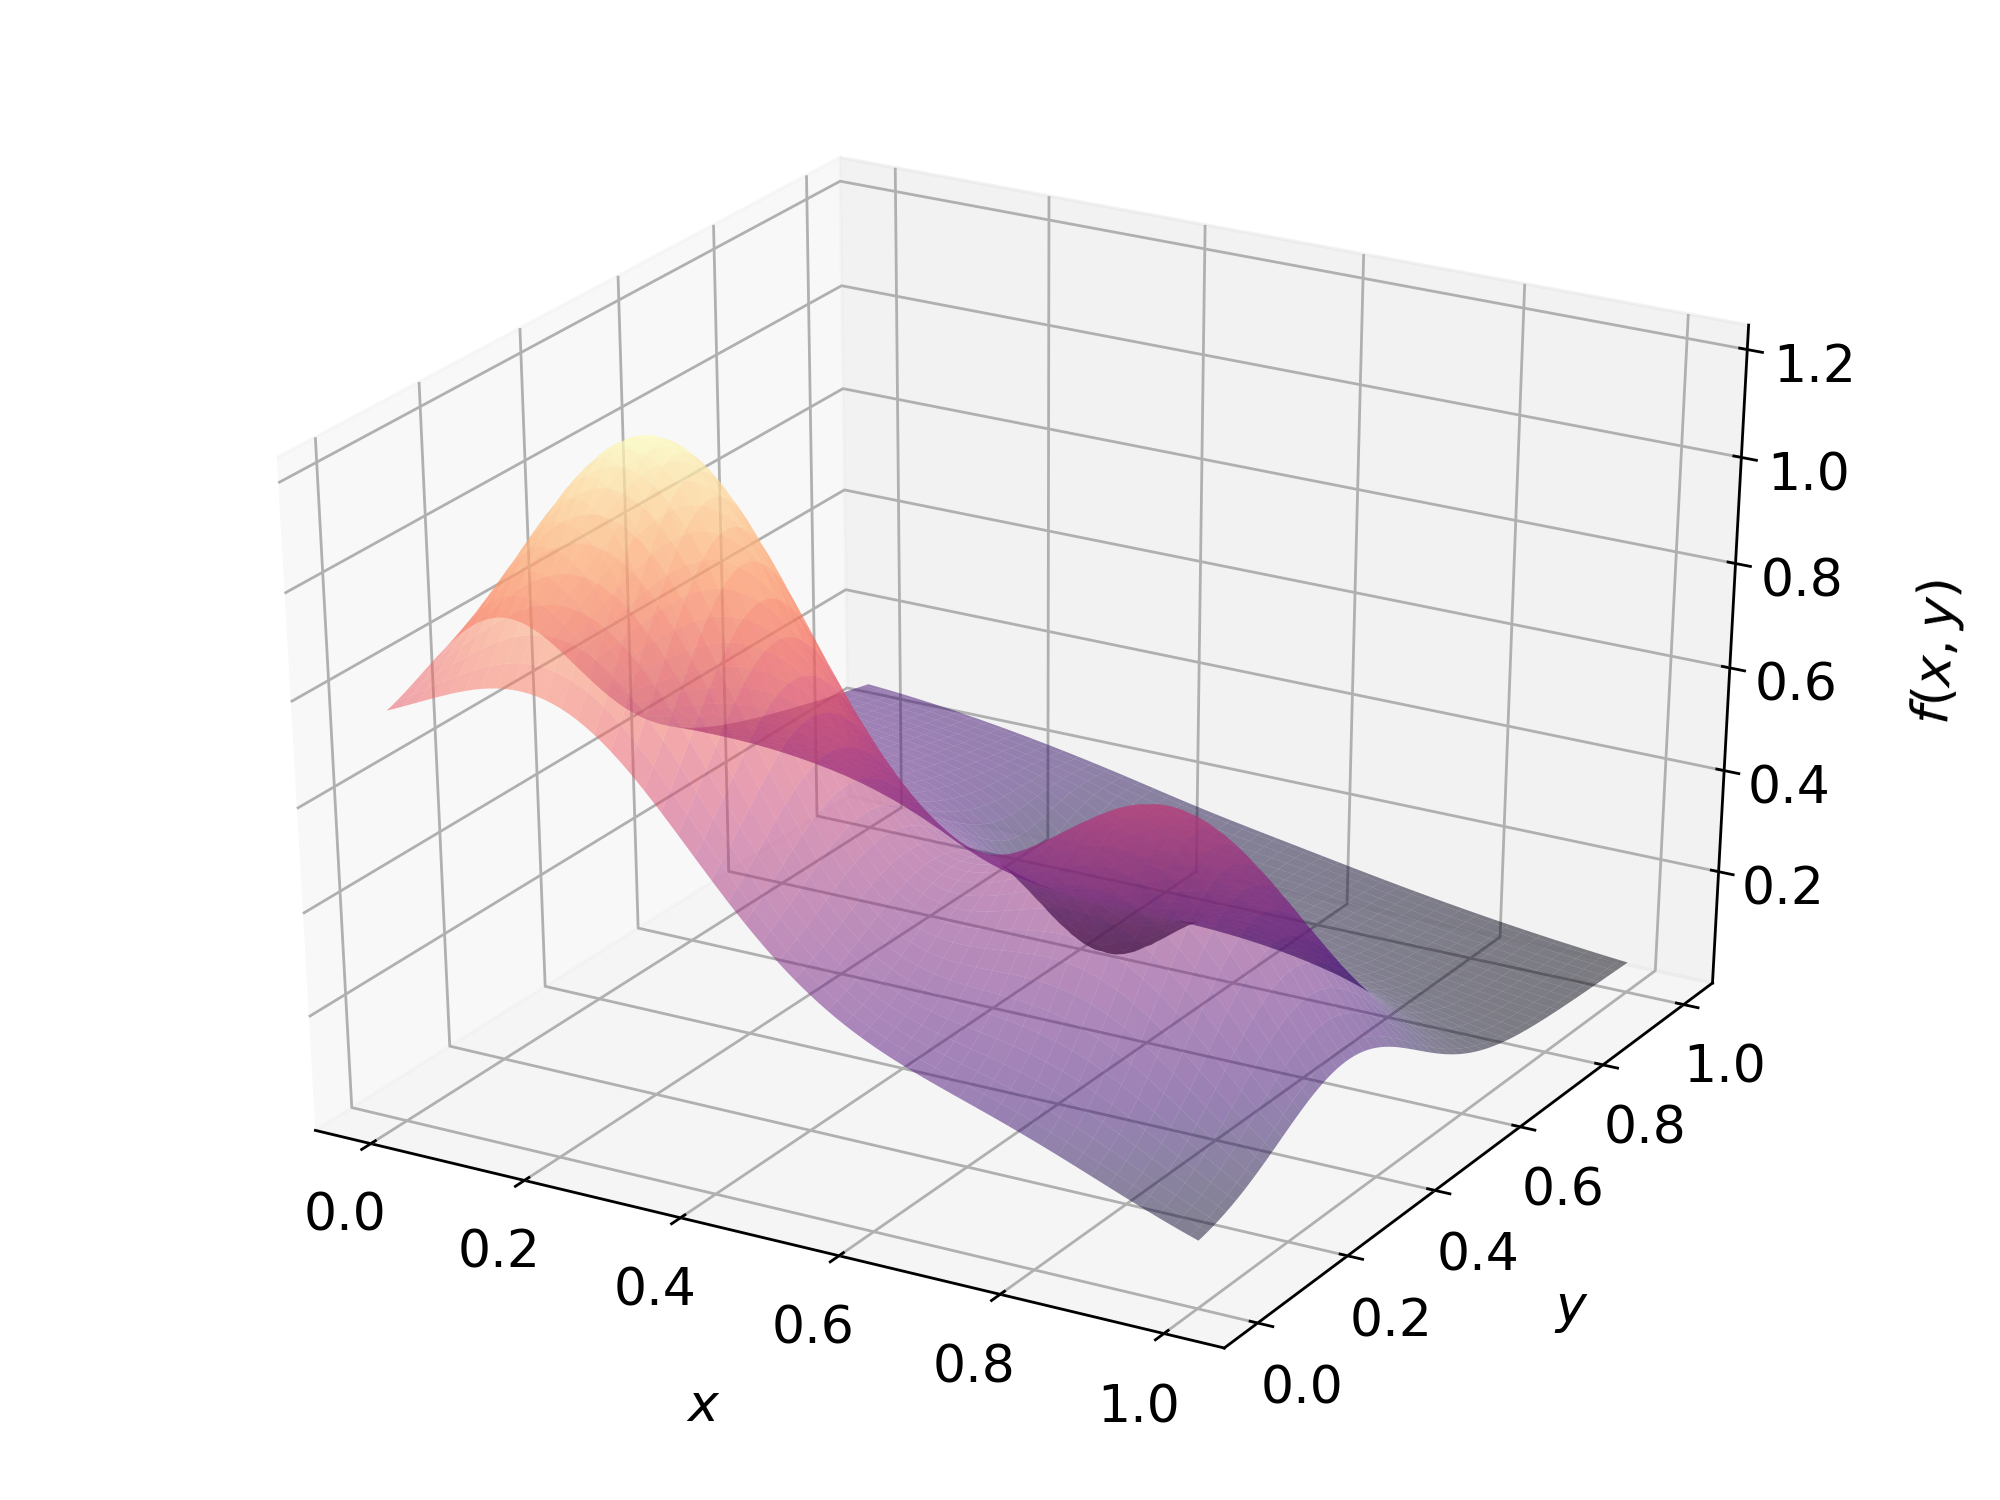
\includegraphics[width = 0.5\textwidth, center]{Franke.png}
	\caption{The \textit{Franke function} for $x$ and $y$ values ranging from zero to one. \label{fig_Franke}}
\end{figure}

In addition, we will also be adding \textit{Gaussian noise} to each value $f(x,y)$, such that we are left with values as seen in Figure \ref{fig_Franke_noise}.

\begin{figure}[H]
	\centering
	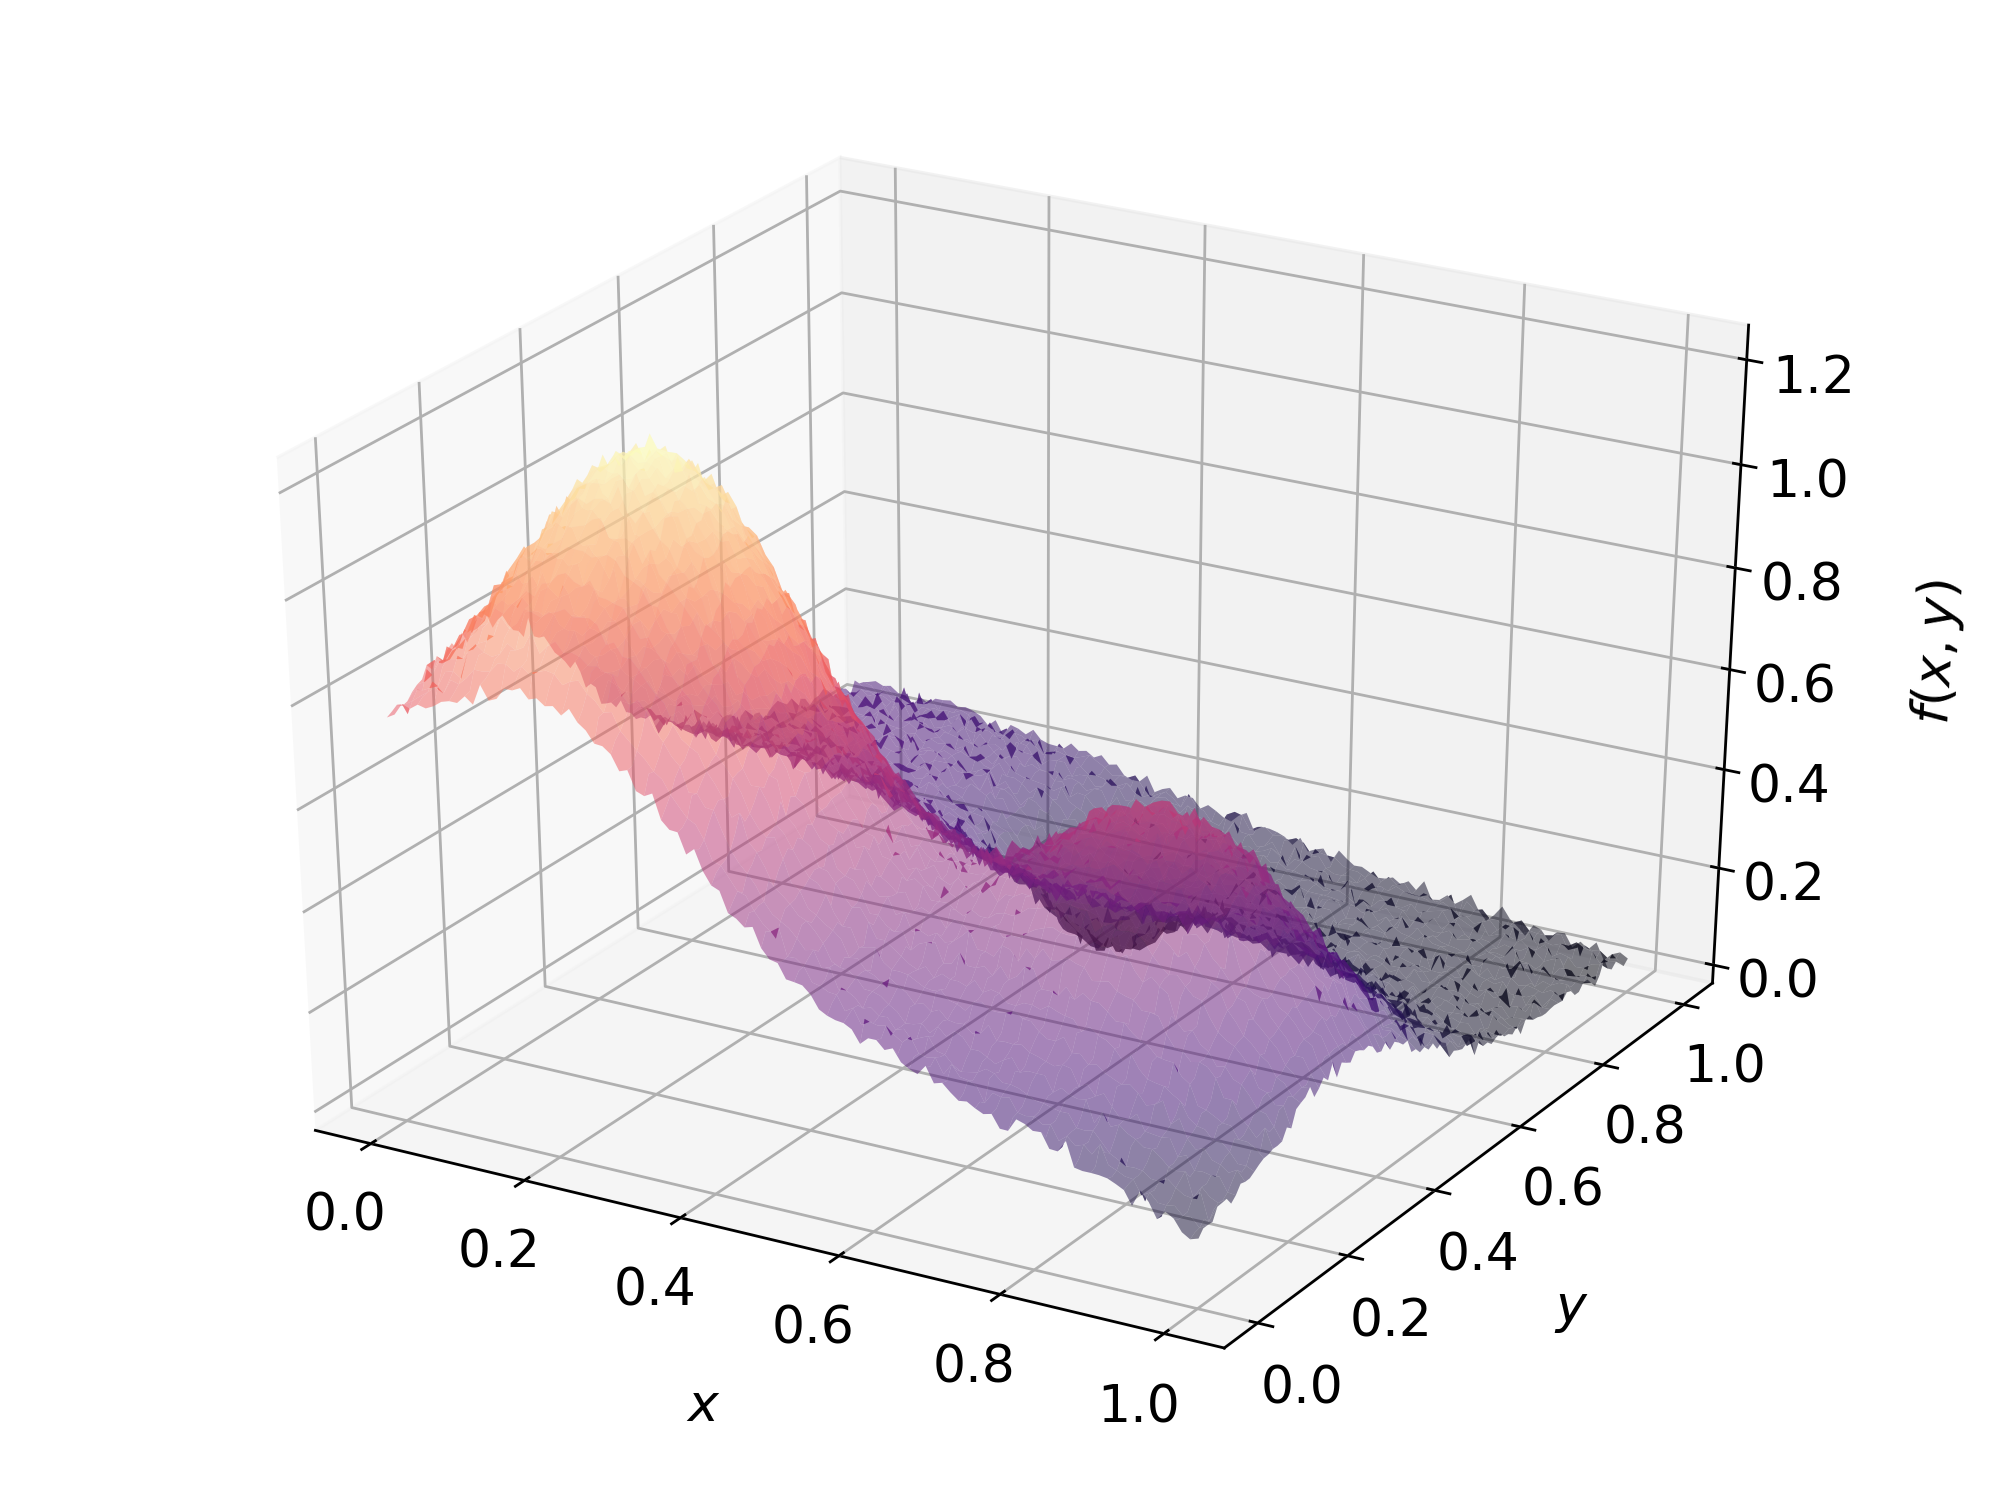
\includegraphics[width = 0.5\textwidth, center]{Franke_noise.png}
	\caption{The \textit{Franke function} for $x$ and $y$ values ranging from zero to one, with a Gaussian noise $N(0,0.01)$\label{fig_Franke_noise}}
\end{figure}

\section*{Method}

\subsection*{Mean Squared Error}

To get a measure of success with respect to the implemented method and parameters, we can calculate the mean difference in the squares of each measured output $y_i$ and their respective predicted outputs $\hat{y}_i$:

\begin{equation*}
MSE(\mathbf{y}, \mathbf{\hat{y}}) = \frac{1}{N} \sum_{i=1}^{N} (y_i - \hat{y}_i)^2 = \mathbb{E}\left[(\mathbf{y}-\hat{\mathbf{y}})^{2}\right]
\end{equation*}

The lower the $MSE$, the closer the polynomial approximation is to the original dataset.  If it is too low, however, we run the risk of overfitting our dataset, which is not desireable either – fortunately, this not an issue within the scope of this report.

\subsection*{R\textsuperscript{2} Score}

Another measure of success is the \textit{coefficient of determination}, colloquially known as the $R^2$ score, is given by the following expression:

\begin{equation*}
R^2 = 1 - \frac{\sum_{i=1}^N (y_i - \hat{y}_i)^2 }{\sum_{i=1}^N (y_i - \bar{y}_i)^2 }
\end{equation*}

The closer $R^2$ is to one, the closer the polynomial approximation is to the input/output dataset, although a perfect score can once again arise due to overfitting just as in the case of the $MSE$.

\section*{Results}

\section*{Discussion}

\section*{Conclusion}

\bibliography{bib}{}
\bibliographystyle{ieeetr}
\end{multicols*}{2}
\end{document}